\documentclass[landscape,a0paper,fontscale=0.292]{baposter}
%\usepackage[english]{babel}
\usepackage[vlined]{algorithm2e}
\usepackage{times}
\usepackage{calc}
\usepackage{url}
\usepackage{graphicx}
\usepackage{amsmath}
\usepackage{amssymb}
\usepackage{relsize}
\usepackage{multirow}
\usepackage{booktabs}
\usepackage{epstopdf}

\usepackage{graphicx}
\usepackage{multicol}
\usepackage[T1]{fontenc}
\usepackage{ae}
\usepackage{multirow}
\usepackage{rotating}


\graphicspath{{images/}}

\DeclareMathOperator*{\argmax}{arg\,max}
\DeclareMathOperator*{\argmin}{arg\,min}

\newcommand{\x}{\mathbf{x}}
\newcommand{\y}{\mathbf{y}}
\newcommand{\h}{\mathbf{h}}
\newcommand{\w}{\mathbf{w}}

 %%%%%%%%%%%%%%%%%%%%%%%%%%%%%%%%%%%%%%%%%%%%%%%%%%%%%%%%%%%%%%%%%%%%%%%%%%%%%%%%
 %%%% Some math symbols used in the text
 %%%%%%%%%%%%%%%%%%%%%%%%%%%%%%%%%%%%%%%%%%%%%%%%%%%%%%%%%%%%%%%%%%%%%%%%%%%%%%%%
 % Format
 \newcommand{\RotUP}[1]{\begin{sideways}#1\end{sideways}}


 %%%%%%%%%%%%%%%%%%%%%%%%%%%%%%%%%%%%%%%%%%%%%%%%%%%%%%%%%%%%%%%%%%%%%%%%%%%%%%%%
 % Multicol Settings
 %%%%%%%%%%%%%%%%%%%%%%%%%%%%%%%%%%%%%%%%%%%%%%%%%%%%%%%%%%%%%%%%%%%%%%%%%%%%%%%%
 \setlength{\columnsep}{0.7em}
 \setlength{\columnseprule}{0mm}


\definecolor{colorRed}{RGB}{0,50,255}%{120,120,120}


%%%%%%%%%%%%%%%%%%%%%%%%%%%%%%%%%%%%%%%%%%%%%%%%%%%%%%%%%%%%%%%%%%%%%%%%%%%%%
%% Begin of Document
%%%%%%%%%%%%%%%%%%%%%%%%%%%%%%%%%%%%%%%%%%%%%%%%%%%%%%%%%%%%%%%%%%%%%%%%%%%%%
\begin{document}
%%%%%%%%%%%%%%%%%%%%%%%%%%%%%%%%%%%%%%%%%%%%%%%%%%%%%%%%%%%%%%%%%%%%%%%%%%%%%
%% Here starts the poster
%%---------------------------------------------------------------------------
%% Format it to your taste with the options
%%%%%%%%%%%%%%%%%%%%%%%%%%%%%%%%%%%%%%%%%%%%%%%%%%%%%%%%%%%%%%%%%%%%%%%%%%%%%
\begin{poster}{
 % Show grid to help with alignment
 grid=false,
 %Number of columns
 columns=4,
 % Column spacing
 colspacing=0.7em,
 % Color style
 headerColorOne=colorRed,
 borderColor=colorRed,
 % Format of textbox
 textborder=roundedsmall,
 % Format of text header
 headerborder=closed,
 headershape=smallrounded,
 headershade=plain,
 headerheight=0.16\textheight,
 headerFontColor=white,
 boxshade=none,
 background=none,
 bgColorOne=cyan!10!white}
 % Eye Catcher
 { 
    \begin{tabular}{c}
      
\includegraphics{logo/CVPRLogo} \\
    \end{tabular}
 }
 % Title
 {\sc\Huge WELDON: Weakly Supervised Learning of \\ \vspace{3mm} Deep Convolutional Neural Networks  \vspace{0.1cm}}
 % Authors
 {Thibaut DURAND, Nicolas THOME, Matthieu CORD \vspace{0.1cm}\\
 {\small Sorbonne Universit\'{e}s, UPMC Univ Paris 06, LIP6, Paris, France}
 } % University logo
 {
    \begin{tabular}{c}
    %  \includegraphics[height=0.07\textheight]{logo_LIP6} \\ %\vspace{0.1cm} 
      \includegraphics[height=0.048\textheight]{logo_upmc}  \\
      \\
      \hspace{-10mm}
      
\includegraphics[height=0.075\textheight]{logo/dga.jpg} \hspace{2mm}
      
\includegraphics[height=0.075\textheight]{logo/cnrs} 
    \end{tabular}
    
 }
 

 
 
 
 

%%%%%%%%%%%%%%%%%%%%%%%%%%%%%%%%%%%%%%%%%%%%%%%%%%%%%%%%%%%%%%%%%%%%%%%%%%%%%%
\headerbox{Context}{name=context,column=0,row=0,span=1}{
%%%%%%%%%%%%%%%%%%%%%%%%%%%%%%%%%%%%%%%%%%%%%%%%%%%%%%%%%%%%%%%%%%%%%%%%%%%%%%


\textbf{Goal:} image classification or ranking
 
$\triangleright$ Learning of deep CNN on small datasets

$\triangleright$ How to transfer on datasets with complex scenes?

$\triangleright$ Problem: invariance (scale, translation)

 \begin{tabular}{cc}
\includegraphics[width=3.5cm]{005831}
& 
\includegraphics[width=3.5cm]{008895} 
\\
{\em OK for centered object} & {\em KO for ``natural'' image}
\end{tabular}

\vspace{1mm}

$\triangleright$ Efficient transfer: needs bounding boxes
 
%$\triangleright$ Supervision: full annotations ({\em e.g.} BB) expensive

$\triangleright$ Full annotations expensive $\Rightarrow$ weak supervision
%Weakly Supervised Learning (WSL) framework 

~~ $\triangleright$ Select relevant regions $\rightarrow$ better prediction

~~ $\triangleright$ Baseline model: Latent SVM (LSVM)

%$\triangleright$ End-to-end training 

\vspace{2mm}
\textbf{Contributions}

$\triangleright$ New region aggregation strategy

$\triangleright$ Structured ranking AP loss for WSL %Loss to optimize Average Precision

$\triangleright$ Fully convolutional architecture 

$\triangleright$ Experimental validation on 6 datasets

}

% %%%%%%%%%%%%%%%%%%%%%%%%%%%%%%%%%%%%%%%%%%%%%%%%%%%%%%%%%%%%%%%%%%%%%%%%%%%%%%
%   \headerbox{Fully $\rightarrow$ Weakly Deep}{name=model,column=0,below=context}{
% %%%%%%%%%%%%%%%%%%%%%%%%%%%%%%%%%%%%%%%%%%%%%%%%%%%%%%%%%%%%%%%%%%%%%%%%%%%%%%
% 
% $\triangleright$ Standard deep architecture: VGG16
% 
% $\triangleright$ Problem: fixed-size image
% 
% $\triangleright$ Adapt architecture to WSL
% 
% ~~ $\triangleright$ Fully connected layer $\rightarrow$ convolution layer 
% 
% ~~~~~ $\triangleright$ Sliding window approach / shared features
% 
% ~~ $\triangleright$ Spatial aggregation 
% 
% ~~~~~ $\triangleright$ Perform object localization prediction
% 
% 
% }

%%%%%%%%%%%%%%%%%%%%%%%%%%%%%%%%%%%%%%%%%%%%%%%%%%%%%%%%%%%%%%%%%%%%%%%%%%%%%%
  \headerbox{Region Aggregation}{name=region,column=0,below=context, above=bottom}{
%%%%%%%%%%%%%%%%%%%%%%%%%%%%%%%%%%%%%%%%%%%%%%%%%%%%%%%%%%%%%%%%%%%%%%%%%%%%%%

\textbf{Baseline:} max aggregation [1] (MIL, LSVM)

\vspace{1mm}

\textbf{Our MANTRA aggregation} [2]
%\textbf{Negative evidence scoring}

$\triangleright$ \texttt{max} + \texttt{min} pooling (negative evidence)

~~ $\triangleright$ \texttt{max}: indicator of the \textbf{presence} of the class

~~ $\triangleright$ \texttt{min}: indicator of the \textbf{absence} of the class


\vspace{-2mm}

\begin{center}
 \begin{tabular}{cc}
\includegraphics[width=3.2cm]{002269_street_bbox_2}
& 
\includegraphics[width=3.2cm]{002269_highway_bbox_2}
\\
\textbf{street} model & \textbf{highway} model
\end{tabular}
\end{center}


\textbf{Our WELDON aggregation} 

$\triangleright$ MANTRA extension to multiple regions
%\textbf{Top instance aggregation}
%
%$\triangleright$ Single region to multiple high scoring regions:
\vspace{-2.5mm}
\begin{equation*}
 \max \rightarrow \frac{1}{k} \sum_{i=1}^k i\text{-th} \max \quad\quad\quad
 \min \rightarrow \frac{1}{k} \sum_{i=1}^k i\text{-th} \min
\end{equation*}

\vspace{-3mm}
$\triangleright$ More robust to outliers

}


%%%%%%%%%%%%%%%%%%%%%%%%%%%%%%%%%%%%%%%%%%%%%%%%%%%%%%%%%%%%%%%%%%%%%%%%%%%%%%
  \headerbox{WELDON Architecture for Classification}{name=reso_results,column=1,row=0,span=2}{
%%%%%%%%%%%%%%%%%%%%%%%%%%%%%%%%%%%%%%%%%%%%%%%%%%%%%%%%%%%%%%%%%%%%%%%%%%%%%%
  
\begin{center}
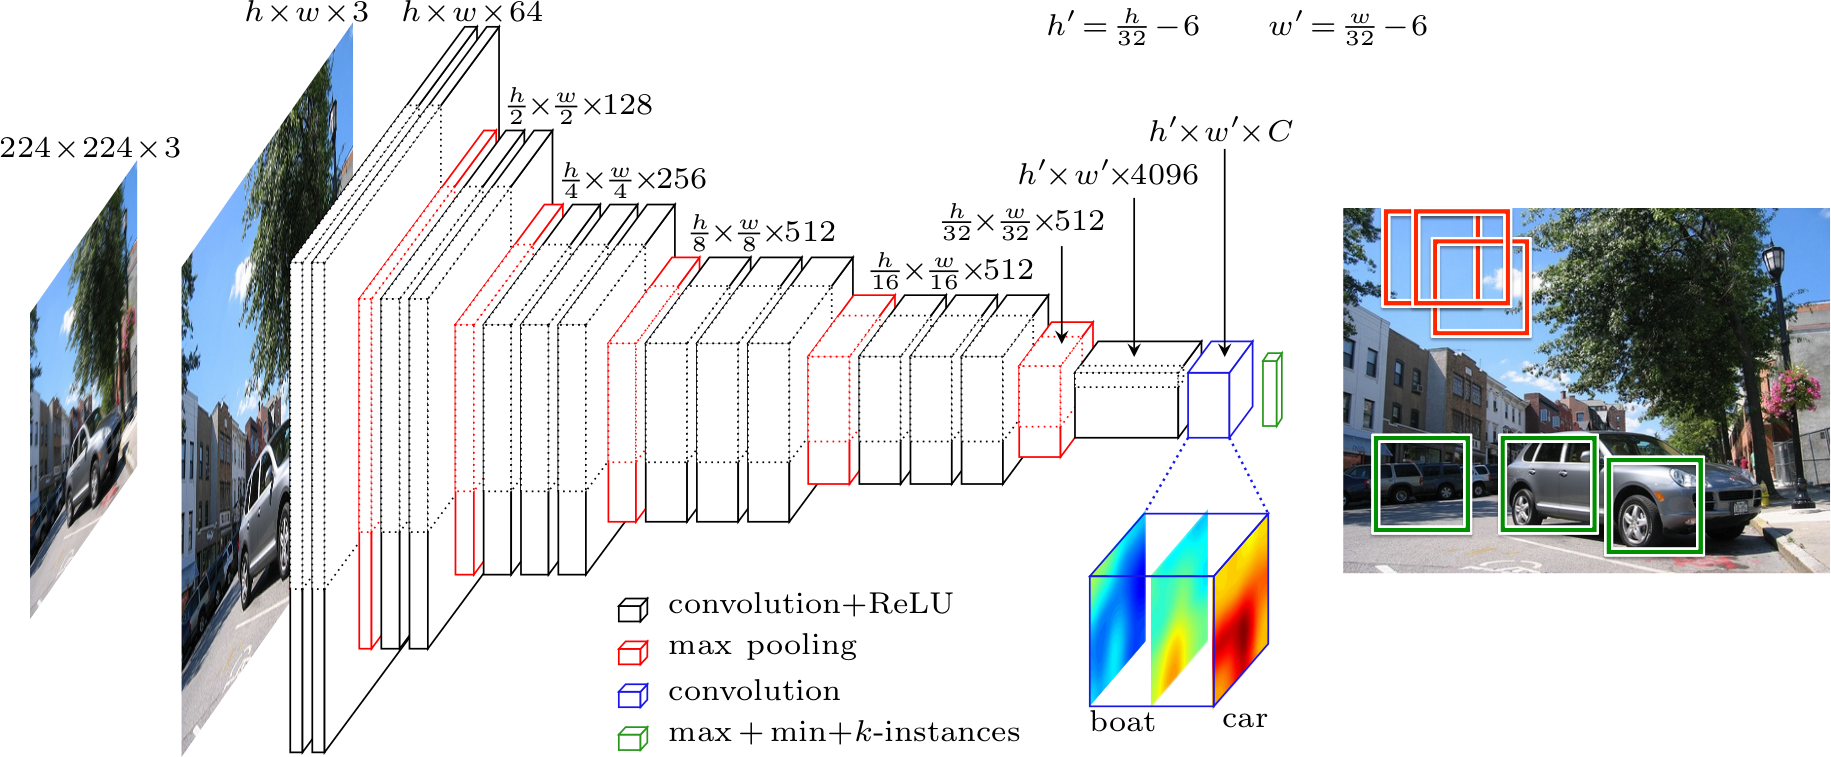
\includegraphics[width=16cm]{archi_weldon2.png}
\end{center}

\vspace{-3mm}
\begin{minipage}[t]{8cm}

$\triangleright$ Fully connected layer $\rightarrow$ convolution layer 

~~ $\triangleright$ Sliding window approach / shared features

\end{minipage} \hfill 
\begin{minipage}[t]{8cm}

$\triangleright$ Spatial aggregation 

~~ $\triangleright$ Object localization prediction

\end{minipage}

}

%%%%%%%%%%%%%%%%%%%%%%%%%%%%%%%%%%%%%%%%%%%%%%%%%%%%%%%%%%%%%%%%%%%%%%%%%%%%%%
  \headerbox{Experiments}{name=lr-cnn,column=1,span=2,below=reso_results,above=bottom}{
%%%%%%%%%%%%%%%%%%%%%%%%%%%%%%%%%%%%%%%%%%%%%%%%%%%%%%%%%%%%%%%%%%%%%%%%%%%%%%

% \begin{center}
% \begin{tabular}{cccccc}
% \hspace{-3.5mm}
%  \includegraphics[height=1.94cm]{000013} & \hspace{-4mm}
%  \includegraphics[height=1.94cm]{003006} & \hspace{-4mm}
%  \includegraphics[height=1.94cm]{2012_004308} & \hspace{-4mm}
%  \includegraphics[height=1.94cm]{COCO_7} & \hspace{-4mm}
%  \includegraphics[height=1.94cm]{15scene} & \hspace{-4mm}
%  \includegraphics[height=1.94cm]{bookstore} \\
%  \hspace{-4mm} VOC 2007 & \hspace{-4mm} VOC 2012 & \hspace{-4mm} VOC12 Action & \hspace{-4mm} COCO & \hspace{-4mm} 15 Scene & \hspace{-4mm} MIT67 
% \end{tabular}
% \end{center}


\begin{minipage}[t]{8cm}

%\vspace{-13mm}

$\triangleright$ VGG16 pre-trained on ImageNet

$\triangleright$ Multi-scale: 8 scales (Object Bank fusion)

\vspace{-3mm}

\begin{center}
\includegraphics[height=3cm]{multiscale_image_heatmap2} 
\end{center}

\vspace{-1mm}

\begin{tabular}{|l|c|c|}
\cline{2-3}
\multicolumn{1}{l|}{Multi-label (mAP)}	& VOC 2007 	& VOC 2012 \\
\hline
VGG16 			& 84.5 	& 82.8 	\\
%SPP net 		& 82.4 	&  		\\
Deep WSL MIL [1]		&  	& 81.8 	\\
%MANTRA [2]	& 85.8	&  		\\
\hline
WELDON			& \textbf{90.2} & \textbf{88.5} \\
\hline
\multicolumn{3}{c}{} \vspace{-3.5mm} \\
\cline{2-3}
\multicolumn{1}{l|}{Multi-label (mAP)}	& VOC12 Action 	& COCO\\
\hline
VGG16 			& 67.1	& 59.7 \\
Deep WSL MIL [1] 		&  & 62.8 \\
\hline
WELDON			& \textbf{75.0}	& \textbf{68.8} \\
\hline
\multicolumn{3}{c}{} \vspace{-3.5mm} \\
\cline{2-3}
\multicolumn{1}{l|}{Multi-class (acc)}	& 15 Scene 		& MIT67 \\
\hline
VGG16  			& 91.2	& 69.9 	\\
MOP CNN [4]		&	& 68.9	\\
%MANTRA [2]			& 93.3	& 76.6	\\
Negative parts [3]		&	& 77.1 	\\
\hline
WELDON 		& \textbf{94.3} 	& \textbf{78.0} \\
\hline
\end{tabular}

\end{minipage} \hfill 
\begin{minipage}[t]{8cm}

\vspace{-3mm}

\begin{tabular}{ccc}
 \includegraphics[height=1.94cm]{003006} & \hspace{-4mm}
 \includegraphics[height=1.94cm]{COCO_7} & \hspace{-4mm}
 \includegraphics[height=1.94cm]{mit67_livingroom}
 \\
 VOC 07/12 & \hspace{-4mm} COCO & \hspace{-4mm} MIT67 
\end{tabular}

$\triangleright$ Analysis of improvements (mono-scale)

\begin{tabular}{cccc|cc}
\texttt{max} & +k=3 & +\texttt{min} & +AP & VOC07 & VOCAct \\ 
\hline
\checkmark & & & & 83.6&   53.5\\ \hline
\checkmark & \checkmark & & & 86.3 & 62.6  \\ \hline
\checkmark & & \checkmark & & 87.5 & 68.4  \\ \hline
\checkmark & & \checkmark & \checkmark & 88.4 & 71.7 \\ \hline
\checkmark & \checkmark & \checkmark & & 87.8 & 69.8 \\ \hline
\checkmark & \checkmark & \checkmark & \checkmark & \textbf{88.9} & \textbf{72.6} \\ 
\hline
\end{tabular}

% \vspace{1mm}
% $\triangleright$ Impact of the number or regions $k$

\begin{tabular}{cc}
\hspace{-3mm} \includegraphics[width=3.8cm]{k_instances_mit6710.png} & \hspace{-3mm} \includegraphics[width=3.8cm]{k_instances_15scene10.png}
\end{tabular}


{
\scriptsize
[1] Oquab et al. Is object localization for free? {\em CVPR}, 2015.

[2] Durand et al. MANTRA. {\em ICCV}, 2015.

[3] Parizi et al. Automatic discovery of parts. {\em ICLR}, 2015.

[4] Gong et al. Multi-scale orderless pooling. {\em ECCV}, 2014.

}

\end{minipage}


}



%%%%%%%%%%%%%%%%%%%%%%%%%%%%%%%%%%%%%%%%%%%%%%%%%%%%%%%%%%%%%%%%%%%%%%%%%%%%%%
  \headerbox{Learning}{name=learning,column=3,row=0}{
%%%%%%%%%%%%%%%%%%%%%%%%%%%%%%%%%%%%%%%%%%%%%%%%%%%%%%%%%%%%%%%%%%%%%%%%%%%%%%

$\triangleright$ Stochastic gradient descent training

$\triangleright$ Back-propagation of the \textbf{selected windows} 

%\vspace{2mm}
\begin{tabular}{cc}
\hspace{-3mm} \includegraphics[width=3.9cm]{learning_car} & \hspace{-4mm} \includegraphics[width=3.9cm]{learning_boat} \\
Class {\em car} is present & Class {\em boat} is absent 
\end{tabular}
%\vspace{-2mm}

$\triangleright$ Optimized ranking metrics (Average Precision)

~~ $\triangleright$ Surrogate upper-bound loss definition

~~ $\triangleright$ Generalized MANTRA ranking instantiation

%~~ $\triangleright$ Exact and efficient (loss-augmented) inference
}

%%%%%%%%%%%%%%%%%%%%%%%%%%%%%%%%%%%%%%%%%%%%%%%%%%%%%%%%%%%%%%%%%%%%%%%%%%%%%%%
%  \headerbox{Optimizing Ranking Metrics}{name=ranking,column=3,below=learning}{
%%%%%%%%%%%%%%%%%%%%%%%%%%%%%%%%%%%%%%%%%%%%%%%%%%%%%%%%%%%%%%%%%%%%%%%%%%%%%%%
%
%$\triangleright$ Goal: predict a ranking matrix
%
%$\triangleright$ Optimized Average Precision
%
%$\triangleright$ Latent structured output formulation [2]
%
%$\triangleright$ Defined a surrogate upper-bound loss
%
%~~ $\triangleright$ Generalized MANTRA ranking instantiation
%
%~~ $\triangleright$ Exact and efficient (loss-augmented) inference
%
%}


%%%%%%%%%%%%%%%%%%%%%%%%%%%%%%%%%%%%%%%%%%%%%%%%%%%%%%%%%%%%%%%%%%%%%%%%%%%%%%
\headerbox{Visual results}{name=visu,column=3,below=learning}{
%%%%%%%%%%%%%%%%%%%%%%%%%%%%%%%%%%%%%%%%%%%%%%%%%%%%%%%%%%%%%%%%%%%%%%%%%%%%%%

\begin{center}
\begin{tabular}{c|c}
\multicolumn{2}{c}{Correct predictions} \\
Correct model & Incorrect model \\
\includegraphics[height=2.2cm]{visus/aero1} & \includegraphics[height=2.2cm]{visus/aero1_bus} \\
\hspace{-4mm} Aeroplane model (1.8) & Bus model (-0.4) \\
\hline
\includegraphics[height=2.2cm]{visus/sofa1}  &  \includegraphics[height=2.2cm]{visus/sofa1_horse} \\
\hspace{-4mm} Sofa model (1.2) & Horse model (-0.6) \\
\hline
\hline 
\multicolumn{2}{c}{Failing example} \\
\includegraphics[height=2.2cm]{images/fail_buffet_gt}  &  \includegraphics[height=2.2cm]{images/fail_buffet_prediction} \\
\hspace{-4mm} Buffet model (1.5) & \small Restaurant kitchen (1.6) \\
\end{tabular}
\end{center}

}

%%%%%%%%%%%%%%%%%%%%%%%%%%%%%%%%%%%%%%%%%%%%%%%%%%%%%%%%%%%%%%%%%%%%%%%%%%%%%%
\headerbox{Latent Variables Models}{name=ouverture,column=3,above=bottom,below=visu}{
%%%%%%%%%%%%%%%%%%%%%%%%%%%%%%%%%%%%%%%%%%%%%%%%%%%%%%%%%%%%%%%%%%%%%%%%%%%%%%

LSSVM: $\max_{h \in \mathcal{H}} f(x,y,h) $  (maximization)

HCRF: $\sum_{h \in \mathcal{H}} \exp(f(x,y,h))$  (marginalization)

WELDON: $\sum_{h \in \Omega \subseteq \mathcal{H}} f(x,y,h) $

}

\end{poster}%
%
\end{document}
